\documentclass{article}
\usepackage{float} % Add this line
% Language setting
% Replace `english' with e.g. `spanish' to change the document language
\usepackage[english]{babel}

% Set page size and margins
% Replace `letterpaper' with`a4paper' for UK/EU standard size
\usepackage[letterpaper,top=2cm,bottom=2cm,left=3cm,right=3cm,marginparwidth=1.75cm]{geometry}

% Useful packages
\usepackage{amsmath}
\usepackage{graphicx}
\usepackage{titlesec} % Added for section title formatting
\usepackage[colorlinks=true, allcolors=blue]{hyperref}

% Define section title format
\titleformat{\section}[hang]{\normalfont\Large\bfseries}{}{0em}{--~}

% Redefine section and subsubsection numbering
\renewcommand{\thesection}{}
\renewcommand{\thesubsection}{}
\renewcommand{\thesubsubsection}{}

\title{CPE 301 Embedded Systems Design Final Project}
\author{Mason Haines, Austin Jarolimek, Samuel Mouradian }
\date{\today}
\begin{document}
\maketitle


\section{Introduction}
This lab project focuses on developing a cooling system, also known as a swamp cooler, using the Arduino 2560 microcontroller and sensors from a standard Arduino kit. The goal is to build a sudo-functional cooler capable of cooling and humidifying air. To automate cooling using an Arduino Mega 2560, integrate sensors like a water level sensor and a DHT11 for environmental monitoring, along with actuators such as a stepper motor for vent control and a fan for cooling. Use Arduino libraries and directly manipulate register values for precise control and display information on an LCD screen. Include a real-time clock module for logging events. System states manage continuous monitoring, vent control, and motor activation, transitioning between IDLE, ERROR (for low water levels), and RUNNING (during cooling). This setup optimizes automation and control for efficient cooling processes.


\subsection{Equipment}
\begin{itemize}
    \item Arduino Mega 2560
    \item USB programming cable
    \item Resistors
    \item Breadboards
    \item Jumper Kit
    \item Female to Male Wires
    \item LCD Screen
    \item DHT11 Temp Humidity Sensor
    \item Water Level Detection Sensor
    \item LEDs
    \item Potentiometer
    \item Buttons
    \item Power Supply Module
    \item 9 Volt Battery
    \item 3-6 V DC Motor
    \item L293D Motor Driver
    \item Stepper Moter (28BY J-48)
    \item Stepper Motor Driver Module
    \item Fan

\end{itemize}

% Define section title format for "Part X" sections
\titleformat{name=\section,numberless}[hang]{\normalfont\Large\bfseries}{}{0em}{--~}


\section{Component Experimental Design Requirements}
\renewcommand{\thesubsubsection}{} % Remove numbering before Experimental Design

   
\subsection{Design Requirements}    
\begin{enumerate}
    \item \textbf{Water Level Sensor:}
    \begin{itemize}
        \item Utilize the water level sensor from the kit for monitoring water levels. Threshold detection can be achieved using either interrupt-based comparator methods or ADC sampling without relying on the ADC library.
    \end{itemize}

    \item \textbf{Stepper Motor:}
    \begin{itemize}
        \item Control the vent direction using a stepper motor, which can be operated via buttons and/or a potentiometer to adjust the vent's orientation. Leverage Arduino libraries for stepper motor control.
    \end{itemize}

    \item \textbf{LCD Screen:}
    \begin{itemize}
        \item Display essential messages on the LCD screen using the Arduino library.
    \end{itemize}

    \item \textbf{RTC Module:}
    \begin{itemize}
        \item Employ the real-time clock module for event reporting purposes, integrating Arduino library functionalities.
    \end{itemize}

    \item \textbf{DHT11 temperature/humidity sensor:}
    \begin{itemize}
        \item Integrate the DHT11 temperature/humidity sensor for real-time environmental monitoring, utilizing the Arduino library for sensor data acquisition.
    \end{itemize}

    \item \textbf{Fan and Motor:}
    \begin{itemize}
        \item Use the provided kit motor and fan blade for the fan motor. Ensure to connect these components using the separate power supply board to prevent damage to the Arduino's output circuitry.
    \end{itemize}
\end{enumerate}

\section{State Descriptions}

\begin{itemize}
    \item \textbf{All States:}
    \begin{itemize}
        \item Utilize the real-time clock to log state transitions and vent position changes via the Serial port.
    \end{itemize}

    \item \textbf{All States except DISABLED:}
    \begin{itemize}
        \item Continuously monitor and display humidity and temperature readings on the LCD screen, updating once per minute.
        \item Respond to changes in vent position control.
        \item The stop button should deactivate the fan motor (if running) and transition the system to the DISABLED state.
    \end{itemize}

    \item \textbf{DISABLED:}
    \begin{itemize}
        \item Illuminate the YELLOW LED.
        \item Cease temperature and water level monitoring.
        \item Utilize an ISR to monitor the start button.
    \end{itemize}

    \item \textbf{IDLE:}
    \begin{itemize}
        \item Log precise transition timestamps using the real-time clock.
        \item Continuously monitor water levels and transition to an error state if levels are insufficient.
        \item Activate the GREEN LED.
    \end{itemize}

    \item \textbf{ERROR:}
    \begin{itemize}
        \item Deactivate the motor and prevent activation regardless of temperature.
        \item Use a reset button to return to the IDLE state if water levels are restored above the threshold.
        \item Display an error message on the LCD screen.
        \item Illuminate the RED LED while deactivating other LEDs.
    \end{itemize}

    \item \textbf{RUNNING:}
    \begin{itemize}
        \item Activate the fan motor.
        \item Transition to the IDLE state once temperatures drop below the set threshold.
        \item Transition to the ERROR state if water levels become critically low.
        \item Illuminate the BLUE LED.
    \end{itemize}
\end{itemize}



\section{Final Project Pictures} 
\begin{figure}[H]
    \centering
    \includegraphics[angle=0,width=0.7\textwidth]{Circuit Design.png}
    \caption{Circuit design schematic built on Cirkit Designer.}
    \label{fig:1}
\end{figure}

\begin{figure}[H]
    \centering
    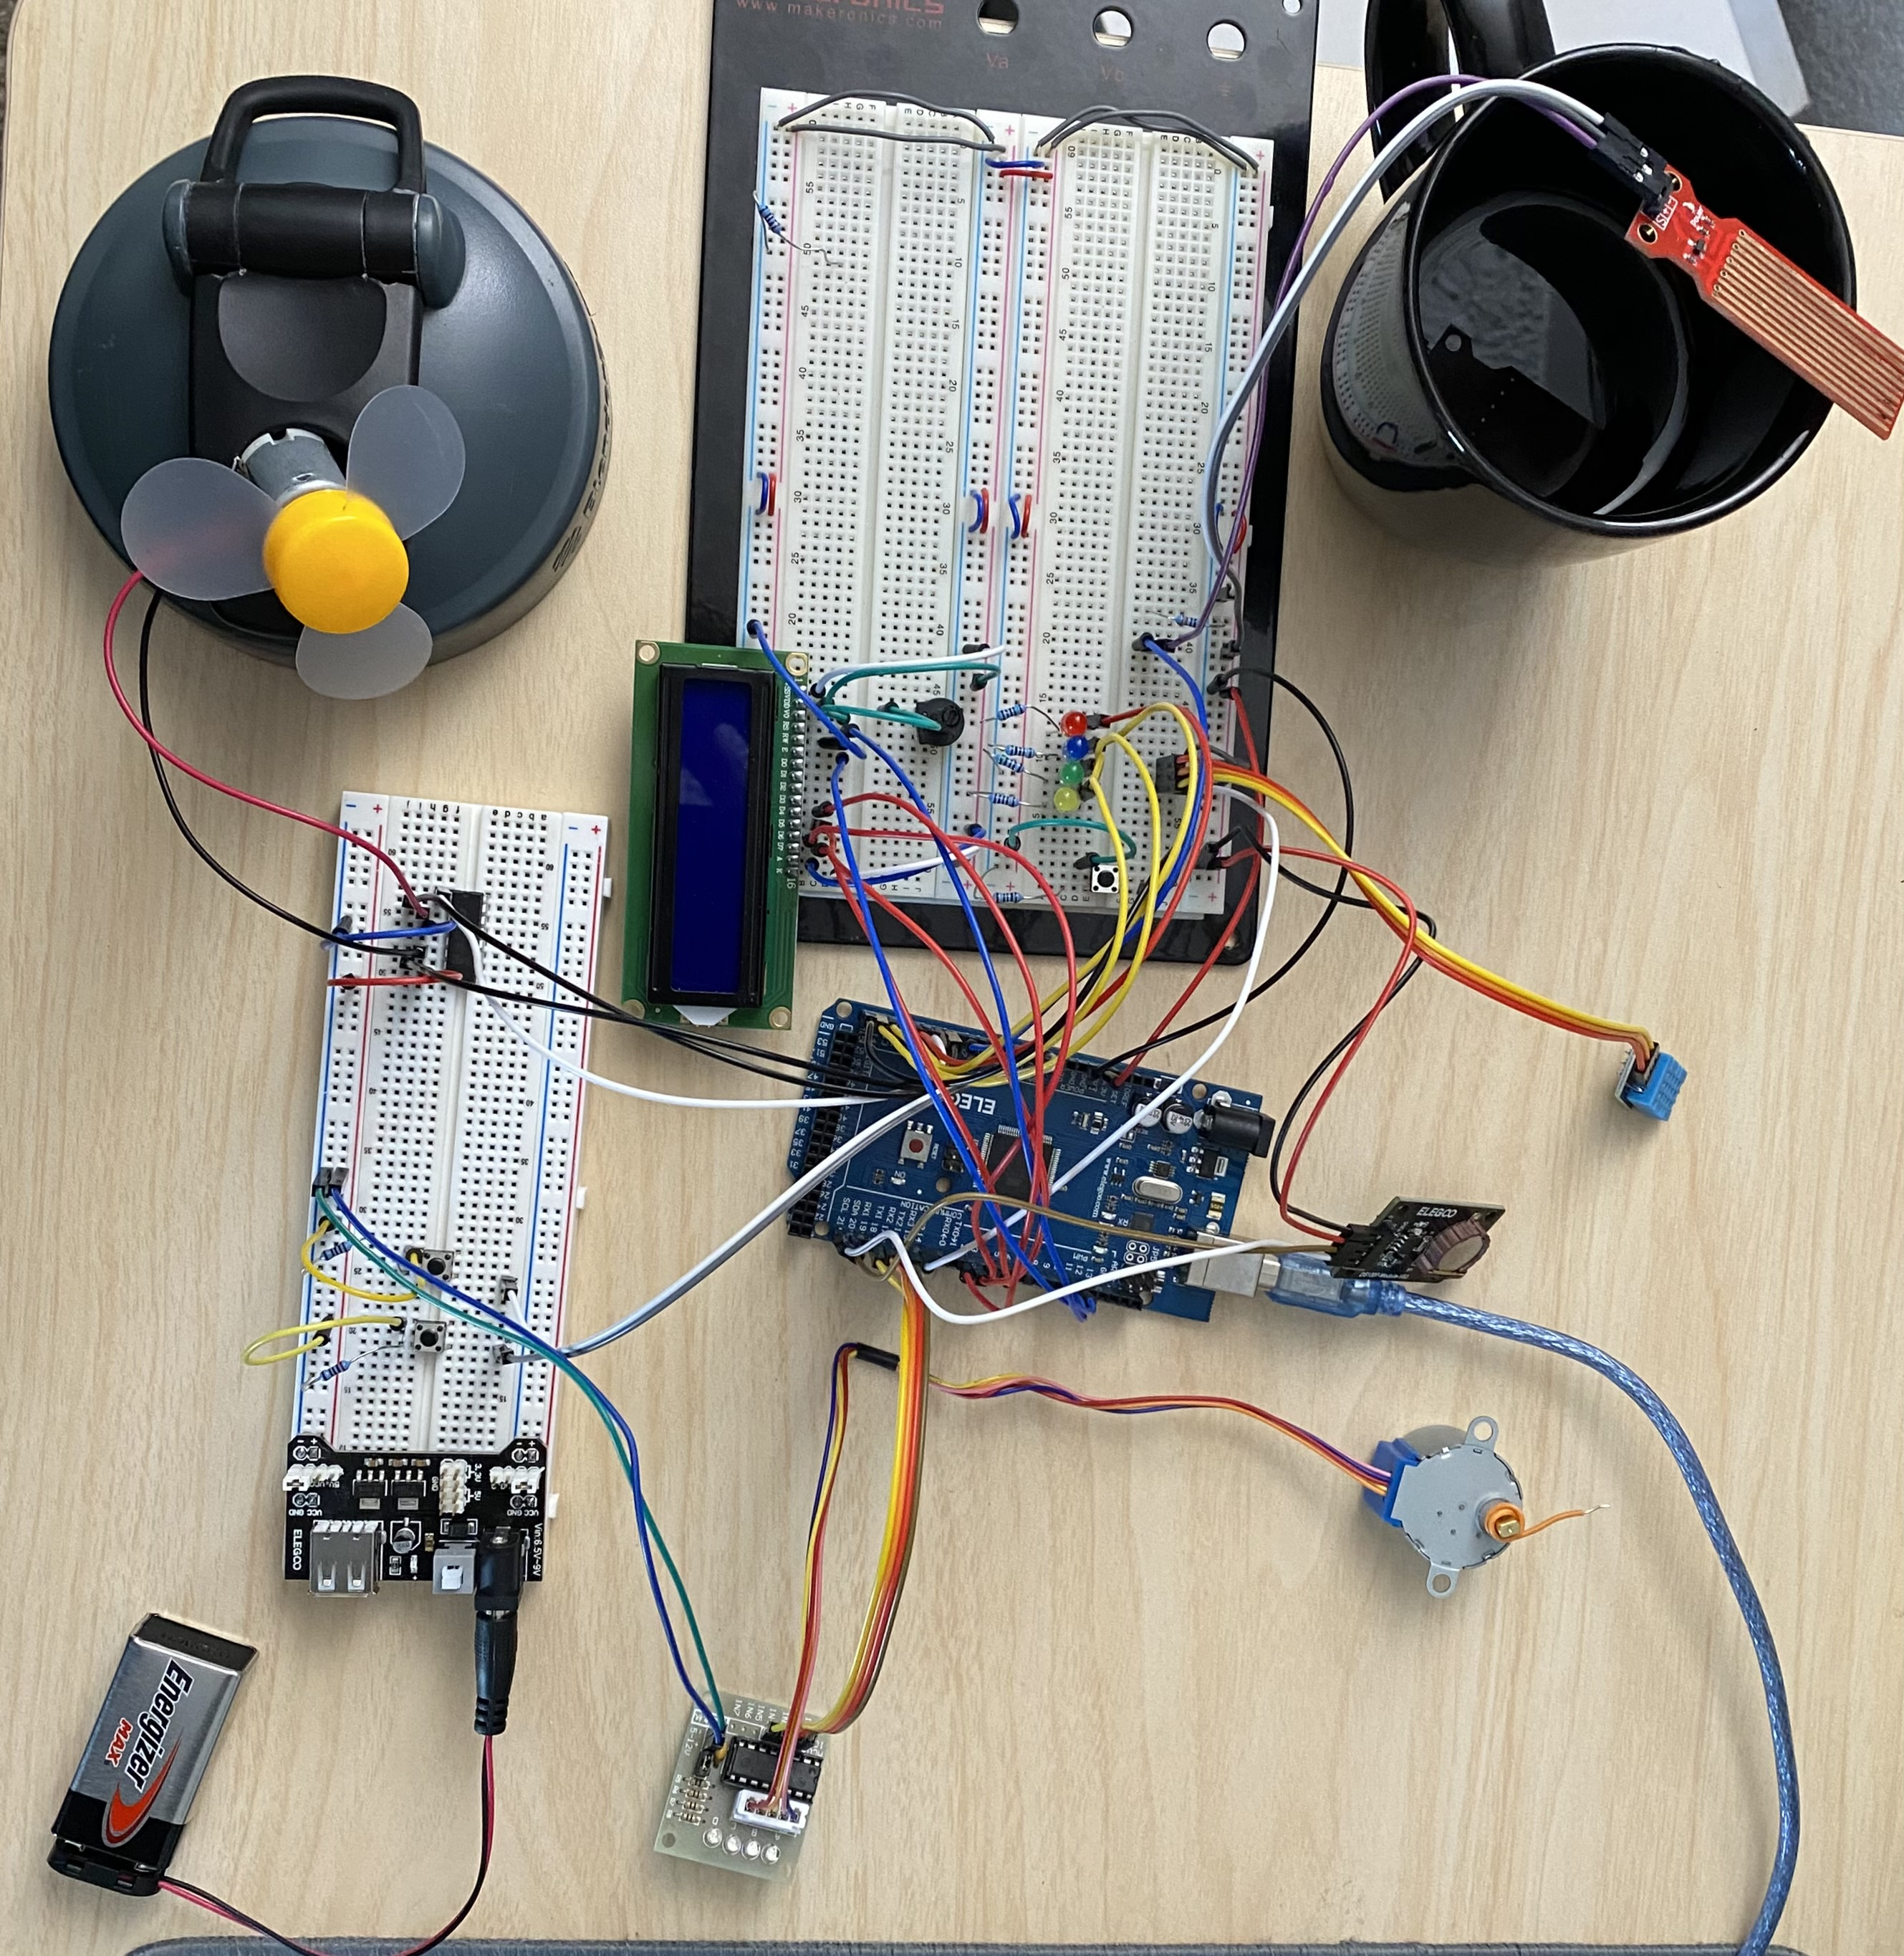
\includegraphics[angle=0,width=0.7\textwidth]{finallabCircuit.jpg}
    \caption{Final circuit setup.}
    \label{fig:1}
\end{figure}

\section{Contributions}

\begin{itemize}
    \item \textbf{Mason Haines:}
    \begin{itemize}
        \item Fan motor code/circuit
        \item Stepper motor code/circuit
        \item Implemented code modules into driver
    \end{itemize}

    \item \textbf{Austin Jarolimek:}
    \begin{itemize}
        \item Temperature/Humidity sensor code/circuit
        \item Water level sensor code/circuit
        \item Lab write-up and documentation
    \end{itemize}

    \item \textbf{Samuel Mouradian:}
    \begin{itemize}
        \item My delay code
        \item RTC code/circuit
        \item Circuit design schematic
    \end{itemize}

        \item \textbf{All:}
    \begin{itemize}
        \item Circuit implementation
        \item Final driver debug
        \item ISR implementation
        \item GPIO research
    \end{itemize}
\end{itemize}

\section {References}
\begin{itemize}
    \item \textbf{Component Links:}
    \begin{itemize}
        \item \textbf{DHT11 Temp/Humidity Sensor:} \url{https://www.circuitbasics.com/how-to-set-up-the-dht11-humidity-sensor-on-an-arduino/}
        \item \textbf{Water Level Sensor:} \url{https://arduinogetstarted.com/tutorials/arduino-water-sensor}
        \item \textbf{LCD Display:} \url{https://arduinogetstarted.com/tutorials/arduino-lcd}
        \item \textbf{Stepper Motor:} \url{https://lastminuteengineers.com/28byj48-stepper-motor-arduino-tutorial/}
        \item \textbf{DC Motor:} 
        \url{https://toptechboy.com/arduino-tutorial-37-understanding-how-to-control-dc-motors-in-projects/}
        \item \textbf{Real-Time Clock:} \url{https://howtomechatronics.com/tutorials/arduino/arduino-ds3231-real-time-clock-tutorial/#google_vignette}
    \end{itemize}
        \item\textbf{Github Link:}
    \begin{itemize}
        \item \textbf{Github Repo:} 
        \url {https://github.com/masonhaines/CPE-301-Final-Project-}
        \end{itemize}
\end{itemize}


% pdflatex example.tex

\end{document}
